\documentclass[../main.tex]{subfiles}
%!TEX root = ./appendixFromAnalysisDossier.tex
\graphicspath {{../}}

\begin{document}
\section{Gondola Hinge} \label{appendix:gondolaHinge}

section{Gondola Hinge}
The loading on the gondola hinge by forces $R_{x'}$ and $R_{z''}$ calculated in system modelling section \ref{gondola2ref} will be relatively small. Stress concentration would occur at points A and B shown in Figure \ref{fig:fillethinge}, however to avoid these stress concentrations fillets will be added to the part. 

\begin{figure}[H]
	\centering
	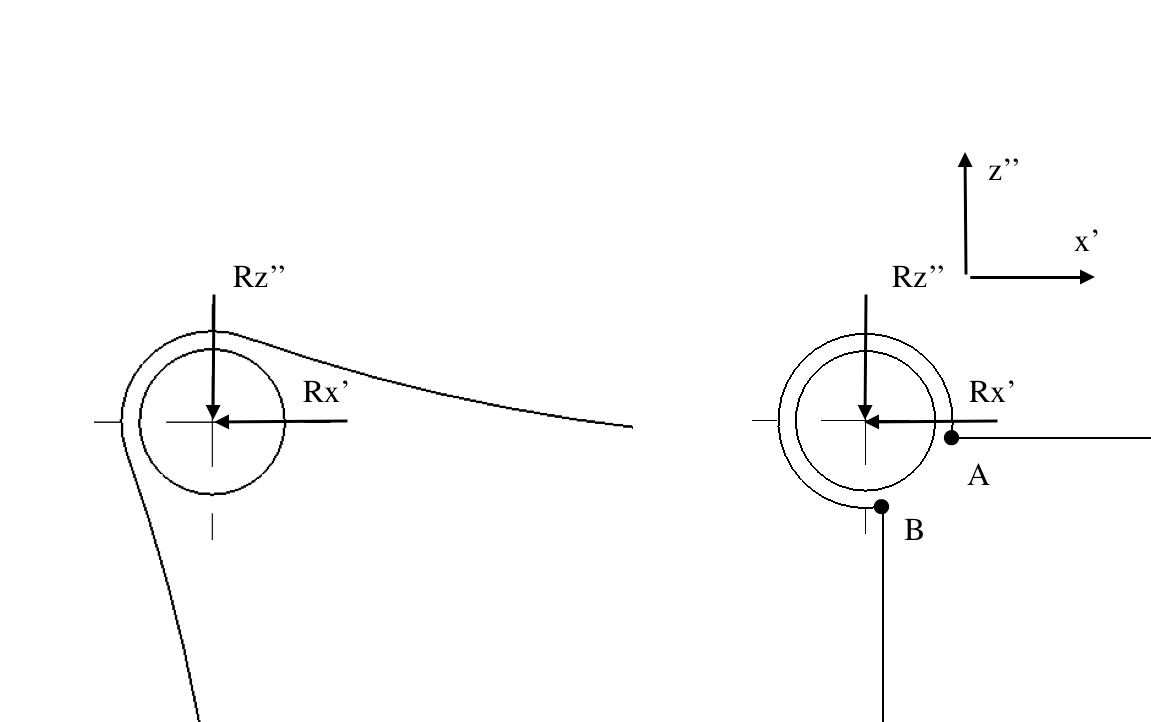
\includegraphics[width=1\textwidth]{img/gondola/filletHinge.PNG}
	\caption{Gondola Hinge Comparison Fillet Vs. No Fillet}
	\label{fig:fillethinge}
\end{figure}

The hinge pin will likely be made of aluminium and the shear stress experienced by the part will not be considerable relative to the strength of the material. 

\end{document}